%Task 4
\documentclass[12pt,a4paper,english]{extarticle}
\usepackage[T1]{fontenc}
\usepackage[utf8]{inputenc}
\usepackage{fourier}
\usepackage{geometry}
\usepackage{multirow}
\geometry{verbose,tmargin=2.2cm,bmargin=2cm,lmargin=2.2cm,rmargin=2cm}
\usepackage{float}
\usepackage{textcomp}
\usepackage{amsmath}
\usepackage{stackrel}
\usepackage{graphicx}
\usepackage{esint}
\usepackage{tikz}
\usetikzlibrary{arrows, shapes.gates.logic.US, calc}
\tikzstyle{branch}=[fill, shape=circle, minimum size=3pt, inner sep=0pt]
\usetikzlibrary{matrix,calc}

\makeatletter

\providecommand{\tabularnewline}{\\}

\usepackage{fancyhdr}
\usepackage{lscape}
\usepackage{amssymb}
\pagestyle{fancy}
\lhead{Electronica III - 22.13}
\chead{TPL1}
\rhead{ITBA}
\renewcommand{\headrulewidth}{1pt}
\renewcommand{\footrulewidth}{1pt}

\makeatother

\usepackage[english]{babel}

\begin{document}

\section*{Task 4}
In this section, there are measured the 
propagation delay, rise time and fall time of
 a 74HC02 logic gate (CMOS tecnology) in 
 several configurations: without load, and with
  a circuit load as shown below.
  
  \begin{figure}[H]
    \begin{centering}
    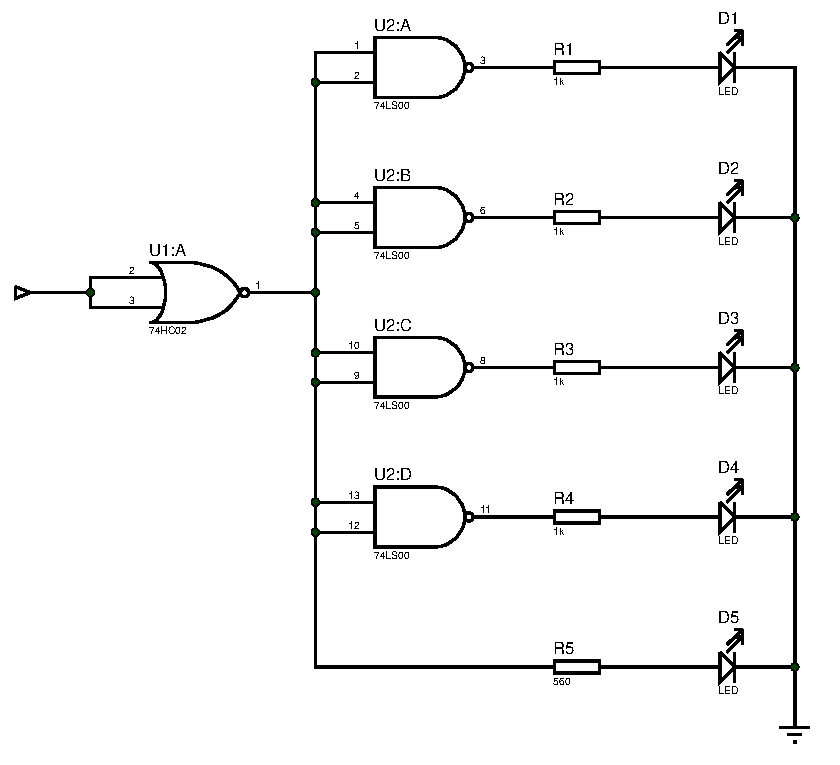
\includegraphics[width=0.7\textwidth]{circuitLED}
    \par\end{centering}
    \caption{Circuit load schematic - Made in Proteus 7.8}
\end{figure}

In the following table are the measured times
for the diferent configurations.

\begin{table}[H]
    \begin{center}
    \begin{tabular}{|c|c|c|c|c|}
    \hline
    CASE & $tpd_{L-H}$ & $tpd_{H-L}$ & $t_r$ & $t_f$\\
    \hline \hline
    Without LOAD & & & &  \\ \hline
    Circuit LOAD & & & & \\ \hline
    Circuit LOAD (100KHz) & & & & \\ \hline
    Circuit LOAD (100KHz with Capacitors) & & & & \\ \hline
    \end{tabular}
    \caption{Measured times}
    \end{center}
\end{table}

CONCLUSIONES DE TEMPERATURA, TIEMPOS Y EL PORQUE
DE USAR 100nF.

\end{document}

